\section{Implementierung}
\subsection{Konventionen bei der Programmierung}
Klassennamen bekommen ein führendes \textbf{T}, Eigenschaften ein 
führendes \textbf{F} und Parameter ein führendes \textbf{A}.\\
Die Klasse mit dem JFrame für die Benutzeroberfläche bekommt ein führendes \textbf{U}.\\
Die verwendete Sprache beim Benennen der erzeugten Wörter im Code ist Englisch.\\
Namen von Packages werden klein geschrieben.

\subsection{Einteilung des Projektes}
Zuerst erstelle ich ein neues Java Projekt mit dem Namen \textbf{bookDB}.\\
In diesem Projekt lege ich dann 3 Packages an:
\begin{itemize}
\item{database}
\item{logic}
\item{userinteface}
\end{itemize}
Im Package database erzeuge ich eine Klasse \textbf{TDatabase}, die für die Verbindung zur Datenbank und zur API zuständige Methoden enthalten soll.\\
Im Package logic erstelle ich für jede Eigenschaft des Buches und für das Buch selbst eine Klasse und eine Klasse, die eine Array Liste dazu enthält.\\
Für die Verarbeitung der Json -Werte wird eine Klasse und eine Klasse mit zugehöriger Liste erstellt.\\
\begin{center}
\begin{table} [htb] % table hat mehr Eigensachaften, z.B. Caption
\centering
\begin{tabular}{  l  r  }
\hline
\rowcolor{cyan}\textbf{Klassenname}&\textbf{Name der Liste}\\
\hline
TAuthor&TAuthorList\\
\rowcolor{lightgray}TGenre&TGenreList\\
TLocation&TLocationList\\
\rowcolor{lightgray}TBook&TBookList\\
TJson&TJsonList\\
\rowcolor{lightgray}TConstants&-\\
\hline
\end{tabular}
\caption{Klassennamen vom Package logic}
\label{tab:Klassennamen_logic}
\end{table}
\end{center}

Außerdem wird eine Klasse \textbf{TConstants} erzeugt, die alle Konstanten für das Programm enthält. Als Programmkonstanten definiere ich:
\begin{itemize}
\item{Name der Datenbank}
\item{Pfad zur Datenbank}
\item{Name der Datei mit dem API -Key}
\item{Pfad zur API -Key Datei}
\item{API -Url}
\end{itemize}

Über den Marketplace der IDE installiere ich den Windowbuilder.\\
Im package userinterface erstelle ich eine Klasse \textbf{UMain}, der mit dem Windowbuilder ein JFrame erzeugt. Hier kann mithilfe des Designers eine Benutzeroberfläche erstellt werden.\\
Zum testen und erstellen von schwierigem Code erstelle ich eine Klasse \textbf{TListTester} als ausführbares Java Programm.

\subsection{Datenstruktur}
\subsubsection{Bibliotheken für Datenbank und JSON}
Damit ich eine Verbindung zu meiner erstellten Datenbank herstellen und SQL Befehle im Code implementieren kann, lade ich Java SQL Treiber aus dem Internet für das Verwenden der JDBC Klassen. \\
\textit{Quelle: http://www.java2s.com/Code/Jar/s/Downloadsqlitejdbc372jar.htm} \\
Für das parsen von JSON lade ich mir ebenfalls eine ausführbare *.jar Datei aus dem Internet.\\
\textit{Quelle: https://jar-download.com/artifacts/org.json}\\
Für den Zugriff auf diese Bibliotheken kopiere ich die 2 *.jar Dateien in meinen Projektordner und in der IDE füge ich diese durch Rechtsklick auf die Dateien zum \textit{Buildpath} des Projektes hinzu.\\
Jetzt müssen noch 2 Einträge in der \textit{module-info} Datei erfolgen:
\begin{itemize}
\item{requires java.sql}
\item{requires java.json}
\end{itemize}
\subsubsection{Datenbank}
Das Programm benötigt zum speichern und wiederherstellen der Benutzerdaten eine Datenbank.
Dafür verwende ich eine lokale \textbf{SQLite} Datenbank.\\
\begin{figure}[h]
\begin{center}
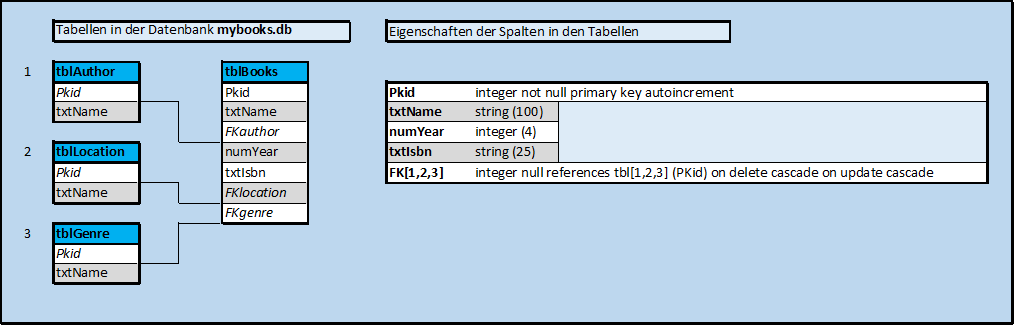
\includegraphics[width=15cm]{img/datenbank.png}
\caption{Entwurf der Datenbank}
\label{datenbank}
\end{center}
\end{figure}

Für das Erstellen der Datenbank \textbf{mybooks.db}, benutze ich das Tool \textit{Database.net}, welches mir im Unterricht bei der RTG bereitgestellt wurde.\\
Über die Eingabemaske erzeuge ich die Tabellen mit einfachen SQLite befehlen.
Die Tabellen \textit{tblAuthor, tblLocation} und \textit{tblGenre} sind einfache \textit{1:n} Beziehungen zur Tabelle \textit{tblBooks}.\\
Beim erzeugen der Fremdschlüssel verwende ich \textit{cascade}, damit beim löschen später die verknüpften Fremdschlüsselbeziehungen mit behandelt werden und dazu nötige SQL Befehle entfallen.\\
\subsubsection{Verbindung zur Datenbank}
Zum Start des Programms soll eine Verbindung zur Datenbank erfolgen und nach Beenden des Programms soll diese getrennt werden.\\
Hierfür erzeuge ich nur eine Instanz der Klasse \textbf{TDatabase} während der Laufzeit des Programms. Mit \textit{public static final} vor dem Klassennamen wird das in JAVA sichergestellt. Zum Verbinden und trennen der Datenbank verwende ich 2 Methoden:
\begin{itemize}
\item{public void connect(){}}
\item{public void disconnect() {}}
\end{itemize}
Die Syntax habe ich im Netz auf der Seite Stackoverflow im Forum recherchiert.
\begin{figure}[h]
\begin{center}
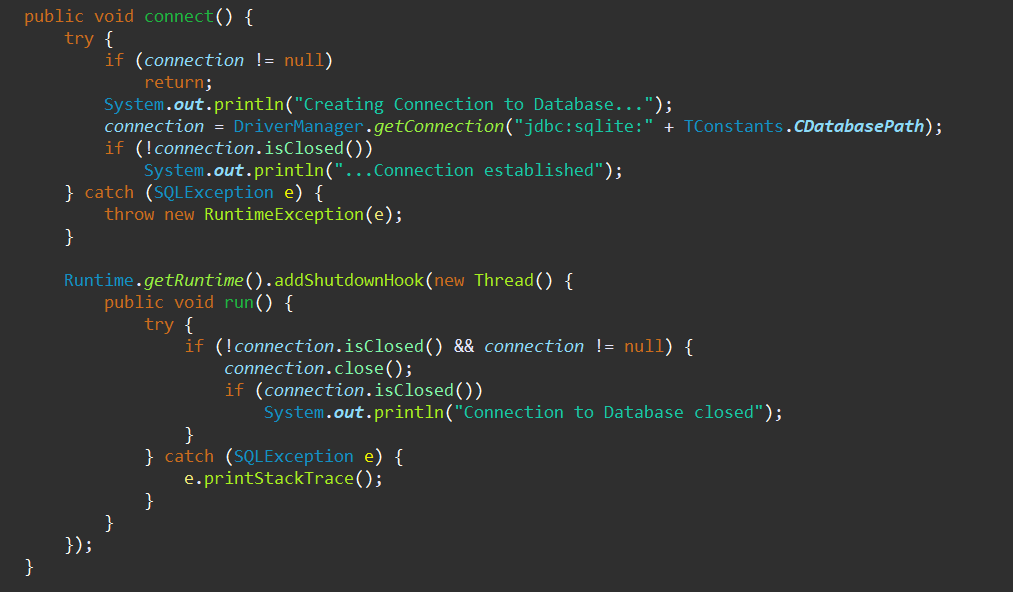
\includegraphics[width=15cm]{img/connect.png}
\caption{Methode connect}
\label{connect}
\end{center}
\end{figure}
\subsubsection{API}
Für die Suche nach Büchern über das Internet benutze ich die \textbf{GoogleBook API}.\\
Auf der Google API Seite richte ich mir unter meinem Benutzerkonto eine neue Applikation ein und lasse mir einen Schlüssel (key) dafür erzeugen. Außerdem beschränke ich diesen \textit{key} auf die GoogleBook API.\\
Diesen Key speichere ich mir lokal in einer Textdatei und lese diesen zu Beginn des Programms mit der Methode \textit{getApiKey} aus.\\
Jetzt können Anfragen über die API-URL (die ich in der Klasse TConstants festlege), gestellt werden. In diesem Fall verwende ich die URL:\\
\textit{https://www.googleapis.com/books/v1/volumes}\\
Darüber werden dann die Suchanfragen gestellt und eine Json wird bei erfolgreicher Verbindung zurückgegeben.\\
Für das holen der JSON verwende ich die Methode\\
\textit{public void getJson() {}}\\
\newpage
Die Syntax habe ich im Netz auf der Seite Stackoverflow im Forum recherchiert.
Alle benötigten Klassen und zugehörige Methoden, wie z.B. die HTTP Verbindung mit SSL Verschlüsselung und der Methode \textbf{GET} aus der Klasse \textbf{java.net.url}, können über Mausklick importiert werden.
\begin{figure}[h]
\begin{center}
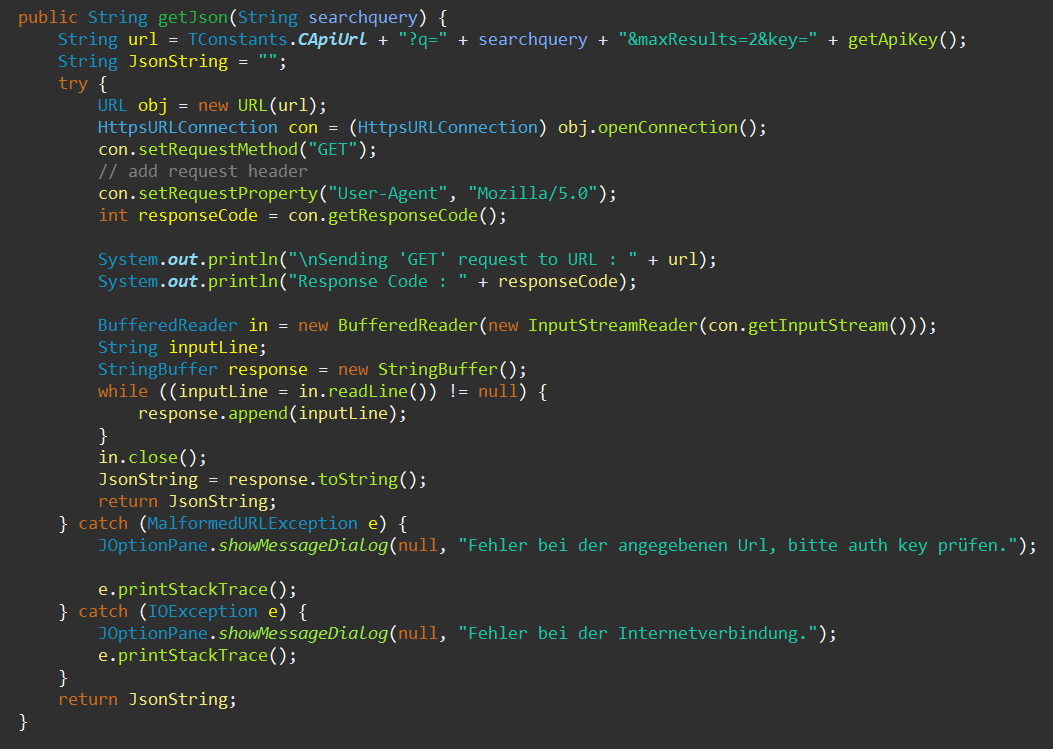
\includegraphics[width=15cm]{img/getjson.png}
\caption{Methode getJson}
\label{getJson}
\end{center}
\end{figure}

\subsection{Logik}
\subsubsection{Konzept}
Zur Umsetzung der Aufgabenstellung im Quellcode benutze ich Objektlisten von Objekten.
Diese Listen werden zu Programmstart in der \textbf{UMain} erstellt und mit den Methoden aus der Logik, die auf die Datenbank zugreifen, gefüllt.\\
Damit setze ich die Darstellung und Bearbeitung der Daten um. Jede Klasse eines Objekts besteht aus Eigenschaften, die Privat deklariert werden. Diese Klassen verfügen über einen Konstruktor in dem die Parameter in dessen Eigenschaften übergeben werden. Mit öffentlichen \textit{getter} und \textit{setter} Methoden kann auf die Eigenschaften zugegriffen werden.\\
Die Objektklassen bekommen jeweils eine \textit{save} und eine \textit{delete} Methode, zum speichern, bzw. löschen der Objekte in der Datenbank.


\subsection{Benutzeroberfläche}
\subsection{Test}

